\subsection{Machine Learning}
\subsubsection{Introduction to Machine Learning}
\begin{enumerate}
    \item A computer is said to learn from examples \textbf{E} in a class of tasks \textbf{T} to improve performance \textbf{P}.\\
        You may understand the \textbf{T,P,E} in a given system as
        \begin{enumerate}
            \item \textbf{T}: Recognition
            \item \textbf{P}: Classification accuracy
            \item \textbf{E}: Labelled images.
        \end{enumerate}
        By giving the system a label, is said to giving the system supervision.
    \item Types of machine learning
    \begin{enumerate}
        \item Supervised Learning \\
        Input:
        \begin{enumerate}
            \item Training Samples
            \item Desired Output
        \end{enumerate}
        Output: A rule that maps input to output.
        \begin{enumerate}
            \item $y$ is continuous : data is regression
            \item $y$ is categorical : data is classification
        \end{enumerate}
        \item Unsupervised Learning \\
        Input: Samples. \\
        Output: Underlying patterns in data.
        \item Reinforcement Learning
        \begin{enumerate}
            \item Given sequence of states \textbf{S} and actions \textbf{A} with delayed rewards \textbf{R}.
            \item Output a policy $\pi(a,s)$
        \end{enumerate}
    \end{enumerate}
    \item Two types of inference
    Inductive: To reach probable conclusions. (Probability and Statistics)
    Deductive: To reach logical conclusions deterministically. (Rule-based reasoning)
\end{enumerate}
\subsubsection{Data Engineering}
\textbf{Types of Data}
\begin{enumerate}
    \item \textbf{NOIR}
    \begin{enumerate}
        \item Nominal Data
        \begin{enumerate}
            \item Lowest level of measurement
            \item Discrete Categories
            \item Measure: Mode, Frequency, Distribution
        \end{enumerate}
        \item Ordinal Data
        \begin{enumerate}
            \item Ordered categories
            \item Relative ranking
            \item Measure: Mode, Frequency distribution, Median
        \end{enumerate}
        \item Interval Data
        \begin{enumerate}
            \item Ordered Categories
            \item Unit measurement and having equal interval
            \item Zero is defined by human (arbitrary)
            \item Measure: Mode, Frequency distribution, Median, Mean, Standard Deviation, Addition/Subtraction
        \end{enumerate}
        \item Ratio Data
        \begin{enumerate}
            \item Most precise and highest level of measurement
            \item Ordered categories
            \item Equal intervals
            \item Natural Zero
            \item Measure: Mode, Frequency distribution, Median, Mean, Standard Deviation, Addition/Subtraction, Multiplication/Division
        \end{enumerate}
    \end{enumerate}
    \item \textbf{Numerical or Categorical}
    \begin{enumerate}
        \item Categorical (Qualitative)
        \begin{enumerate}
            \item Nominal: Unordered categories 
            \item Ordinal: Ordered categories
        \end{enumerate}
        \item Numerical (Quantitative)
        \begin{enumerate}
            \item Discrete: whole numerical values.
            \item Continuous: Can take any value within a range.
            \item Interval: May compute difference but no absolute zero.
            \item Ratio: May compute difference, real zero exists.
        \end{enumerate}
    \end{enumerate}
    \item \textbf{Missing Data} \\
    When there is missing data, you should use a single common code for all missing values.
\end{enumerate}
\textbf{Data wrangling and cleaning}
\begin{enumerate}
    \item \textbf{Data Wrangling}
    \begin{enumerate}
        \item Binary Coding: convert categories into binary form.\\
        Example: $red = [1,0,0]$ $yellow = [0,1,0]$ $green = [0,0,1]$ 
        \item Normalization \\
        Linear Scaling: $\displaystyle x_i = \frac{x_i^{raw}-x^{min}}{x^{max}-x^{min}}, \quad i = 1,2,\ldots,M$ \\
        Z-score standardization: $\displaystyle x_i = \frac{x_i^{raw}-E[X]}{\sigma(X)},\quad i = 1,2,\ldots,M.$
    \end{enumerate}
    \item \textbf{Data Cleaning}\\
    Handling missing features
        \begin{enumerate}
            \item Removing the examples with missing features from the dataset.
            \item Using a learning algorithm that can deal with missing feature values.
            \item Using a data imputation technique.\\
            Method 1: Replace missing value with average value.\\
            $\displaystyle \hat{x}^{(j)} \leftarrow \frac{1}{N} \sum_{i=1}^{N} x_i^{(j)}$ \\
            Method 2: Highlight the missing value, use a value that make the missing value stand out from the majority of dataset.
        \end{enumerate}
    \end{enumerate}
\textbf{Data Integrity and Visualization}
\begin{enumerate}
    \item Data Integrity \\ 
    Make sure that in a numeric column or cells should not accpet any alphabetic data.\\
    A binary entry should only allow binary inputs.
    \item Visualisation \\
    Distribution, Bars, Box-plots.
\end{enumerate}
\subsubsection{Introduction to Linear Algebra, Probability and Statistics}
\textbf{Notations of vectors}
\begin{enumerate}
    \item $\matr{a} = \begin{bmatrix}
        a_1 \\ a_2
    \end{bmatrix}
    = \begin{bmatrix}
        a^{(1)} \\
        a^{(2)}
    \end{bmatrix}
    = \begin{bmatrix}
        2 \\3
    \end{bmatrix}$
    \item  Vector like $a^{(j)}$, the position index $j$ denotes a specific dimension of the vector, the position of an attribute in the list of an attribute in the list.
    \item Vectors can be visualized as in a multi-dimensional space, \textbf{arrows} or \textbf{points}. 
    \item Matrix is defined as $\displaystyle \matr{X} = \begin{bmatrix}
        2 & 4 & 3\\
        21 & -6 & -1 \\
    \end{bmatrix}$
    \item Each row we call it \textbf{sample 1,2,3...} and each columns we call it \textbf{feature 1,2,3...}. 
    \item A Set is an unordered collection of unique elements. E.g. $\mathbb{R}$ includes all numbers from minus infinity to plus infinity.
    \item $\displaystyle \sum$ meaning summation,$\displaystyle \prod$ meaning Product.
\end{enumerate}
\textbf{Systems of Linear Equations}
\begin{enumerate}
    \item \[\beta_1 x_1+\cdots+\beta_m x_m = 0\] 
    If \(\beta_1 x_1+\cdots+\beta_m x_m = 0\) holds for $\beta_1 ,\cdots,\beta_m$ that are not all zero. This is \textbf{Linearly dependent}.\\
    If it only holds \(\beta_1 = \cdots = \beta_m = 0\), this is \textbf{Linearly independent}.
    \item Geometry of dependency and independency
    \begin{figure}[h]
        \centering
        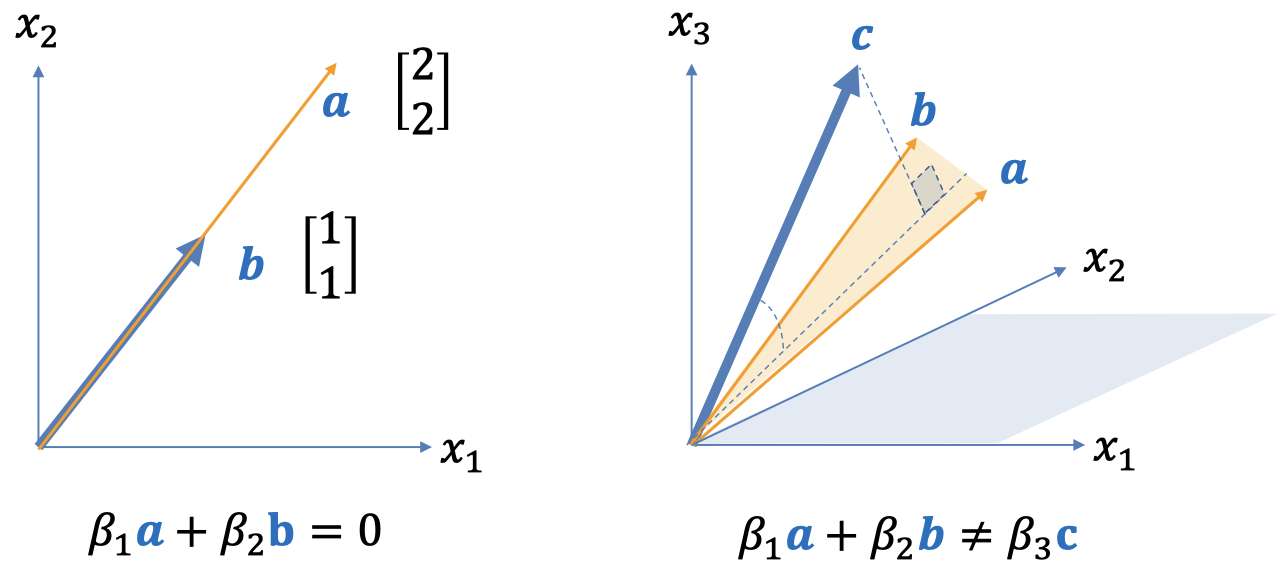
\includegraphics[width=0.70\linewidth]{image/gerolieanr.png}
    \end{figure}
    \item Matrix-vector notation : $\displaystyle \matr{Xw} = \matr{y}$ where \\
    $\matr{X} = \begin{bmatrix}
    x_{1,1} & x_{1,2} & \cdots & x_{1,d} \\
    \vdots & \vdots & \ddots & \vdots \\
    x_{m,1} & x_{m,2} & \cdots & x_{m,d}
    \end{bmatrix}$, $\matr{w} = \begin{bmatrix}
        w_1\\ \vdots \\ w_d
    \end{bmatrix}$, $\matr{y} = \begin{bmatrix}
        y_1\\ \vdots \\ y_m
    \end{bmatrix}$. \\
    Where $\matr{X}$ is the data matrix and $\matr{y}$ is target vector. We are usually asked to calculate $w$ which is the unknown vector of parameters. The rank($\matr{X}$) corresponds to the maximal number of linearly independent columns or rows of X.
\end{enumerate}
\textbf{Causality and Simpsons's paradox}
\begin{enumerate}
    \item Causality \\ 
    The influence by which one event or process contributes to another, The cause is partly responsible for the effect, and the effect is partly dependent on the cause.\\
    \textbf{Randomized Controlled Trial (RCT)}, A study design that randomly assigns participants into an experimental group or a control group.\\
    As the study is conducted, the only expected difference between two groups is the outcome variable being studied.
    \item Correlation \\
    Correlations are useful because they can indicate a predictive relationship that can be exploited in practice.
    \begin{figure}[h]
        \centering
        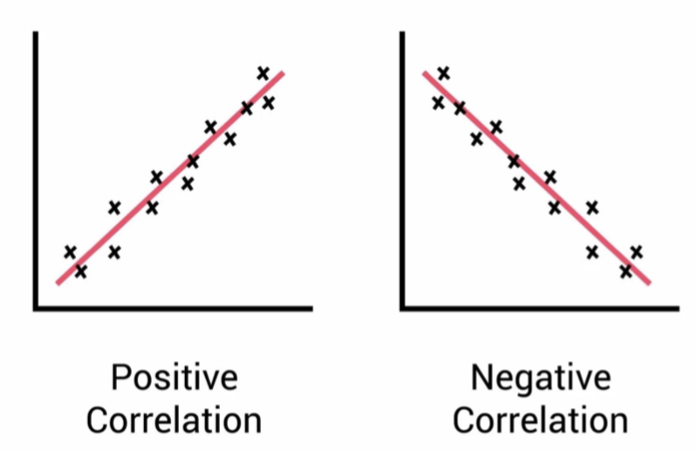
\includegraphics[width=0.75\linewidth]{image/correlation.png}
    \end{figure} \\
    Linear correlation coefficient, $r$, which is also known as the\textit{Pearson correlation Coefficient}. 
    \[r = \frac{\sum_{i=1}^{n} (x_i - \bar{x})(y_i - \bar{y})}
    {\sqrt{\sum_{i=1}^{n} (x_i - \bar{x})^2} \sqrt{\sum_{i=1}^{n} (y_i - \bar{y})^2}}
    = \frac{s_{xy}}{s_x s_y}\]
    \begin{table}[h]
        \centering
        \begin{tabular}{lc}
        \hline
        \textbf{Type of Relationship} & \textbf{Correlation Coefficient (\( r \))} \\
        \hline
        Strong linear relationship & \( r > 0.9 \) \\
        Medium linear relationship & \( 0.7 \leq r \leq 0.9 \) \\
        Weak linear relationship & \( 0.5 < r \leq 0.7 \) \\
        No or doubtful linear relationship & \( 0 < r \leq 0.5 \) \\
        \hline
        \end{tabular}
        \caption{Correlation coefficient and strength of linear relationship}
    \end{table}
    \item Simpson's paradox \\
    Simpson's paradox is a phenomenon in probability and statistics, in which a trend appears in several different groups of data but disappears or reverses when these groups are combined.
\end{enumerate}
\textbf{Random Variable, Bayes' Rule}
\begin{enumerate}
    \item Probability \\
    Sample space $S$, $A$ is a subset of $S$, named an event. \\
    Axioms of Probability
    \begin{enumerate}
        \item $P(A) \geq 0$
        \item $P(S) = 1$
        \item If $A \cap B = \emptyset$, then $P(A \cup B) = P(A) + P(B)$. Otherwise, $P(A \cup B) = P(A) + P(B) - P(A \cap B)$.
    \end{enumerate} 
    Take note in this particular course, use $Pr(\cdot)$ to represent probability symbol.
    \item Discrete Random Variable \\
    Expectation of DRV: \(E(x) \overset{\text{def}}{=} \sum_{i=1}^{k} [x_i \cdot \Pr(X = x_i)]\)
    where $Pr(X = x_i)$ is the probability that $X$ has the value $x_i$ acoording to the PMF.\\
    Standard deviation: \(\sigma \overset{\text{def}}{=} \sqrt{E\left[(X - \mu)^2\right]}\) \\
    Variance: \(\sigma^2 = E\left[(X - \mu)^2\right]\) \\
    \item Continuous Random Variable \\
    Expectation of CRV: \(E[X] \overset{\text{def}}{=} \int_{\mathbb{R}} xf(x)dx\) \\
    Variance: \(\sigma^2 \overset{\text{def}}{=} \int_{\mathbb{R}} (X - \mu)^2 f_X(x) \, dx\) \\
    \item Two Basic Rules
    Sum rule
    \[\Pr(X = x) = \sum_{Y} \Pr(X = x, Y = y_i)\]
    Product rule
    \[\Pr(X = x, Y = y) = \Pr(Y = y | X = x) P(X = x)\]
    \item Bayes' Rule
    \[\Pr(Y = y | X = x) = \frac{\Pr(X = x | Y = y) \Pr(Y = y)}{\Pr(X = x)}\]
\end{enumerate}
\subsubsection{System of Linear Equations}
\textbf{Operations on vectors and Matrices}
\begin{enumerate}
    \item Transpose \\
    \[\matr{x} = \begin{bmatrix}
        x_1 \\
        x_2
    \end{bmatrix} \quad \matr{x}^T = \begin{bmatrix}
        x_1& x_2
    \end{bmatrix}\]
    In python you may use \texttt{numpy} to find out the tranpose or rank of the vector or matrix.
    \begin{minted}[linenos=true]{python}
        import numpy as np
        from numpy.linalg import matrix_rank
        X = np.array([[1, 4, 3], [0, 4, 2], [1, 8, 5]]) 
        print(matrix_rank(X)) #Calculating Rank
        print(X)
        print(X.T) #This is the transpose of X
    \end{minted}
    \item Dot Product or Inner Product of Vectors \\
    $\matr{x}\cdot\matr{y} = \matr{x}^T\matr{y}$\\
    The geometric definition is 
    \[\matr{x}\cdot\matr{y} = ||x||\;||y||\cos{\theta}\]
    where $\theta$ is the angle between $\matr{x}$ and $\matr{y}$, and $||x|| = \sqrt{\matr{x}\cdot\matr{x}}$ is the \textit{Educlidean} length of vector $\matr{x}$.
    \item Matrix-Vector Product 
    \begin{align*}
        \matr{x}^T\matr{W} &= \begin{bmatrix} x_1 & x_2 \end{bmatrix} \begin{bmatrix} W_{1,1} & W_{1,2} & W_{1,3} \\ W_{2,1} & W_{2,2} & W_{2,3} \end{bmatrix}\\
        & = \begin{bmatrix} (x_1 W_{1,1} + x_2 W_{2,1}) & (x_1 W_{1,2} + x_2 W_{2,2}) & (x_1 W_{1,3} + x_2 W_{2,3}) \end{bmatrix}
    \end{align*}
    \item Matrix Inverse \\
    A d-by-d square matrix $\matr{A}$ is invertible (also nonsingular) if there exists a d-by-d square matrix $\matr{B}$ such that $\matr{AB} = \matr{BA} = \matr{I} \text{(identity matrix)}$.
    \[\matr{A}^{-1} = \frac{1}{\det(\matr{A})} \text{adj}(\matr{A})\]
    $\det(\matr{A})$ is the determinant of $\matr{A}$. \\
    $\text{adj}(\matr{A})$ is the adjugate or adjoint of $\matr{A}$.\\
    Take note that $\text{adj}(\matr{A}) = \matr{C}^T$\\
    For $\displaystyle \matr{A} = \begin{pmatrix}
    a_{11} & a_{12} & a_{13} \\
    a_{21} & a_{22} & a_{23} \\
    a_{31} & a_{32} & a_{33}
    \end{pmatrix}$, The cofactor matrix is \\
    $\displaystyle \matr{C} = 
    \begin{pmatrix}
    + & \begin{vmatrix}
    a_{22} & a_{23} \\
    a_{32} & a_{33}
    \end{vmatrix} &
    - & \begin{vmatrix}
    a_{21} & a_{23} \\
    a_{31} & a_{33}
    \end{vmatrix} &
    + & \begin{vmatrix}
    a_{21} & a_{22} \\
    a_{31} & a_{32}
    \end{vmatrix} \\
    - & \begin{vmatrix}
    a_{12} & a_{13} \\
    a_{32} & a_{33}
    \end{vmatrix} &
    + & \begin{vmatrix}
    a_{11} & a_{13} \\
    a_{31} & a_{33}
    \end{vmatrix} &
    - & \begin{vmatrix}
    a_{11} & a_{12} \\
    a_{31} & a_{32}
    \end{vmatrix} \\
    + & \begin{vmatrix}
    a_{12} & a_{13} \\
    a_{22} & a_{23}
    \end{vmatrix} &
    - & \begin{vmatrix}
    a_{11} & a_{13} \\
    a_{21} & a_{23}
    \end{vmatrix} &
    + & \begin{vmatrix}
    a_{11} & a_{12} \\
    a_{21} & a_{22}
    \end{vmatrix}
    \end{pmatrix}$\\
    You may find the inverse of a matrix in python using 
    \begin{minted}[linenos=true]{python}
        import numpy as np
        import numpy.linalg as la
        la.inv(A)
    \end{minted} 
\end{enumerate}
\textbf{Systems of Linear Equations}
\begin{enumerate}
    \item Equations in matrix-vector notation 
    \[\matr{X}\matr{w} = \matr{y}\]
    where
    \[\matr{X} =
    \begin{bmatrix}
    x_{1,1} & x_{1,2} & \cdots & x_{1,d} \\
    \vdots & \vdots & \ddots & \vdots \\
    x_{m,1} & x_{m,2} & \cdots & x_{m,d}
    \end{bmatrix}, \quad
    \matr{w} =
    \begin{bmatrix}
    w_{1} \\
    \vdots \\
    w_{d}
    \end{bmatrix}, \quad
    \matr{y} =
    \begin{bmatrix}
    y_{1} \\
    \vdots \\
    y_{m}
    \end{bmatrix}.\]
    \begin{table}[ht]
    \centering
    \begin{tabular}{l c l}
    \hline
    \textbf{Matrix Type} & \textbf{System Type} & \textbf{Condition} \\
    \hline
    $\matr{X}$ is Square & Even-determined & \( m = d \) (Equal number of equations and unknowns) \\
    $\matr{X}$ is Tall & Over-determined & \( m > d \) (More number of equations than unknowns) \\
    $\matr{X}$ is Wide & Under-determined & \( m < d \) (Fewer number of equations than unknowns) \\
    \hline
    \end{tabular}
    \end{table}
    \item Square or even-determined system: $m=d$ \\
    If $\matr{X}$ is invertible, then the solution can be written as 
    \begin{align*}
        \matr{X}^{-1}\matr{X}\matr{w} &= \matr{X}^{-1}\matr{y} \\
        \hat{\matr{w}} &= \matr{X}^{-1}\matr{y}
    \end{align*}
    \item Over-determined system: $m>d$ \\
    For $\matr{X}$ is a non-square tall matrix, it has no exact solution in general. An approximated solution can be calculated using left-inverse. $\matr{X}^{\dagger}\matr{X} = \matr{I}$. \\
    The left inverse of $\matr{X}$ is given by 
    \[\matr{X}^{\dagger} = (\matr{X}^T\matr{X})^{-1}\matr{X}^T\]
    This will result in
    \begin{align*}
        \matr{X}^{\dagger}\matr{X}\matr{w} &= \matr{X}^{\dagger}\matr{y} \\
        \hat{\matr{w}} &= \matr{X}^{\dagger}\matr{y}
    \end{align*}
    This left-inverse can be calculated in python 
    \begin{minted}[linenos=true]{python}
        def linverse(x):
            xtx = x.T.dot(x)
            if round(la.det(xtx)) == 0:
                return "No solution"
            else:
                return la.inv(xtx).dot(x.T)
    \end{minted}
    \item Under-determined system : $m<d$ \\
    When there are more unknowns than equations, there are infinite numbers of solutions in general. If the right-inverse of $\matr{X}$ exists, we can use it to find a unique constrained solution.\\
    The right inverse of $\matr{X}$ is given by
    \[\matr{X}^{\dagger}=\matr{X}^T(\matr{X}\matr{X}^T)^{-1}\]
    The unique constrained solution can be found using $\matr{w} = \matr{X}^T\matr{a}$
    \begin{align*}
        \matr{X}\matr{w} &= \matr{y} \\
        \matr{X}\matr{X}^T\matr{a} &= \matr{y} \\
        \hat{\matr{a}} & = (\matr{X}\matr{X}^T)^{-1}\matr{y}\\
        \hat{\matr{w}} = \matr{X}^T\matr{a} & = \matr{X}^T (\matr{X}\matr{X}^T)^{-1}\matr{y}
    \end{align*}
    This right-inverse can be calculated in python
    \begin{minted}[linenos=true]{python}
        def rinverse(x):
            xxt = x.dot(x.T)
            if round(la.det(xxt)) == 0:
                return "No solution"
            else:
                return x.T.dot(la.inv(xxt))
    \end{minted}
\end{enumerate}
\textbf{Sets and Functions}
\begin{enumerate}
    \item Intersection : $\{1,3,5,8\}\cap\{1,8,4\} = \{1,8\}$
    \item Union : $\{1,3,5,8\} \cup \{1,8,4\} = \{1,3,4,5,8\}$
    \item Functions \\
    A scalar function can have vector argument E.g. $f(\matr{x}) = x_1+x_2+2x_3$. \\
    A vector function, denoted as $\matr{y} = f(\matr{x})$ is a function that returns a vector $\matr{y}$. \\
    Linear Functions: 
    \begin{itemize}
        \item Homogeneity: $f(\alpha \matr{x}) = \alpha f(\matr{x})$
        \item Additivity: $f(\matr{x}+\matr{y}) = f(\matr{x})+f(\matr{y})$
    \end{itemize}
    Inner product function: \\
    $f(\matr{x}) = a^T \matr{x} = a_1 x_1 + a_2 x_2 + \cdots + a_d x_d$ \\
    Affine function: \\
    $f(\matr{x}) = a^T\matr{x}+b \quad \text{scalar $b$ is called the offset}$
\end{enumerate}
\subsubsection{Least Squares and Linear Regression}
\textbf{Derivative and Gradient}
\begin{enumerate}
    \item Differentiation of a scalar function w.r.t a vector
    \[\frac{d f(\mathbf{x})}{d \mathbf{x}} =\begin{bmatrix}\frac{\partial f}{\partial x_1} \\\vdots \\\frac{\partial f}{\partial x_d}\end{bmatrix}\]
    This is referred to as the gradient of $f(\mathbf{x})$ and often written as $\nabla_{\mathbf{x}}f$.
    \item Differentiation of a vector function w.r.t a vector
    \[\frac{d \mathbf{f}(\mathbf{x})}{d \mathbf{x}} =
    \begin{bmatrix}
    \frac{\partial f_1}{\partial x_1} & \cdots & \frac{\partial f_1}{\partial x_d} \\
    \vdots & \ddots & \vdots \\
    \frac{\partial f_h}{\partial x_1} & \cdots & \frac{\partial f_h}{\partial x_d}
    \end{bmatrix}\]
    The matrix is referred to as the \textbf{Jacobian} of $\mathbf{f(x)}$ \\
    Some Vector-Matrix Differentiation Formulae \\
    \[\frac{d\mathbf{Ax}}{d\mathbf{x}}=\mathbf{A}; \quad \frac{d(\mathbf{b}^T\mathbf{x})}{d\mathbf{x}}=\mathbf{b};\quad \frac{d(\mathbf{y}^T\mathbf{Ax})}{d\mathbf{x}}=\mathbf{A}^T\mathbf{y};\quad \frac{d(\mathbf{x}^T\mathbf{Ax})}{d\mathbf{x}}=(\mathbf{A}+\mathbf{A}^T)\mathbf{x}\]
\end{enumerate}
\textbf{Linear Regression} \\
Linear regression is a popular regression learning algorithm that learns a model which is a linear combination of features of the input example.
\begin{enumerate}
    \item Standard linear regression form
    \[\mathbf{Xw=y},\; \mathbf{X}\in\Re^{ m\times d},\;\mathbf{w}\in\Re^{d\times 1},\; \mathbf{y}\in\Re^{m\times 1}\]
    \[\mathbf{X} = \begin{bmatrix}x_{1,1} & x_{1,2} & \cdots & x_{1,d} \\\vdots & \vdots & \ddots & \vdots \\x_{m,1} & x_{m,2} &\cdots & x_{m,d}\end{bmatrix}, \quad\mathbf{w} = \begin{bmatrix}w_{1} \\\vdots \\w_{d}\end{bmatrix}, \quad\mathbf{y} = \begin{bmatrix}y_{1} \\\vdots \\y_{m}\end{bmatrix}\]
    \item Problem Statement
    \[f_{\mathbf{w},b}(\mathbf{x}) = \mathbf{x}^\top \mathbf{w} + b\]
    The notation $f_{\mathbf{w},b}$ means that the model $f$ is parameterized by two values: $\mathbf{w}$ and $b$.
    \item Objective function\\
    To find the optimal values for $\mathbf{w\*}$ and $b\*$ which minimizes the following expression
    \[\frac{1}{m} \sum_{i=1}^{m} \left( f_{\mathbf{w},b}(\mathbf{x}_i) - y_i \right)^2\]
    $\left( f_{\mathbf{w},b}(\mathbf{x}_i) - y_i \right)^2$ is called \textbf{loss function}: measuring distance between $f_\mathbf{w}(\mathbf{x}_i)$ and $y_i$.
    \item Least Square Regression \\
    Learning : \[\Hat{\mathbf{w}} = (\mathbf{X}^T\mathbf{X})^{-1}\mathbf{X}^T\mathbf{y}\]
    Prediction: \[\Hat{\mathbf{f_w}}(\mathbf{X_{new}}) = \mathbf{X_{new}}\Hat{\mathbf{w}}\]
\end{enumerate}

\subsubsection{Ridge and Polynomial Regression}
\textbf{Ridge Regression}
\begin{equation}
    \Hat{\mathbf{w}} = (\mathbf{X^TX}+\lambda \mathbf{I})^{-1}\mathbf{X^Ty}
\end{equation}
\begin{enumerate}
    \item Primal Form (when m $>$ d)\\
    \(\text{Learning:} \quad \hat{\mathbf{w}} = (\mathbf{X}^\mathsf{T}\mathbf{X} + \lambda \mathbf{I})^{-1} \mathbf{X}^\mathsf{T}\mathbf{y}\) \\
    \(\text{Prediction:} \quad \hat{f}_\mathbf{w}(\mathbf{X}_\text{new}) = \mathbf{X}_\text{new} \hat{\mathbf{w}}\)
    \item Dual Form (when m $<$ d) \\
    \(\text{Learning:} \quad \hat{\mathbf{w}} = \mathbf{X}^\mathsf{T}(\mathbf{X}\mathbf{X}^\mathsf{T} + \lambda \mathbf{I})^{-1} \mathbf{y}\)\\
    \(\text{Prediction:} \quad \hat{f}_\mathbf{w}(\mathbf{X}_\text{new}) = \mathbf{X}_\text{new} \hat{\mathbf{w}}\)
\end{enumerate}
\textbf{Polynomial Regression}
\begin{enumerate}
    \item Primal Form (m $>$ d) \\
    \(\text{Learning:} \quad \hat{\mathbf{w}} = (\mathbf{P}^\mathsf{T}\mathbf{P} + \lambda \mathbf{I})^{-1} \mathbf{P}^\mathsf{T}\mathbf{y}\) \\
    \(\text{Prediction:} \quad \hat{f}_\mathbf{w}(\mathbf{P}(\mathbf{X}_\text{new})) = \mathbf{P}_\text{new} \hat{\mathbf{w}}\)
    \item Dual Form (m $<$ d)\\
    \(\text{Learning:} \quad \hat{\mathbf{w}} = \mathbf{P}^\mathsf{T}(\mathbf{P}\mathbf{P}^\mathsf{T} + \lambda \mathbf{I})^{-1} \mathbf{y}\)\\
    \(\text{Prediction:} \quad \hat{f}_\mathbf{w}(\mathbf{P}(\mathbf{X}_\text{new})) = \mathbf{P}_\text{new} \hat{\mathbf{w}}\)
\end{enumerate}
\newpage
\subsubsection{Over-fitting, bias/variance trade-off}
\textbf{Over-Fitting}\\
Over-fitting occurs when model predicts the training data well, but predicts new data (e.g., from test set) poorly. \\
This could be caused by
\begin{enumerate}
    \item Model too complex for the data.
    \item Too many features but number of training samples too small.
\end{enumerate}
Possible solutions are
\begin{enumerate}
    \item Use simpler models (e.g. lower order polynomial)
    \item Use regularization
\end{enumerate}
\textbf{Under-Fitting}\\
Under-fitting is the inability of trained model to predict the targets in the training set.
This could be caused by
\begin{enumerate}
    \item Model too simple for the data.
    \item Features are not informative enough
\end{enumerate}
Possible solutions are
\begin{enumerate}
    \item Try more complex model
    \item Try to develop more informative features
\end{enumerate}
\textbf{Feature Selection}\\
In order to reduce over-fitting we may use feature selection. \\
Feature selection process
\begin{enumerate}
    \item Feature selection in training set
    \item Fit model using selected features in training set
    \item Evaluate trained model using test set
\end{enumerate}
Note that {\color{red}Do \textbf{NOT} perform feature selection with test data!}\\
\textbf{Regularization} \\
Regularization is an umbrella term that includes methods forcing learning algorithm to build less complex models.\\
The motivations are 
\begin{enumerate}
    \item Solve an ill-posed problem (e.g. estimate 10th order polynomial with just 5 data points)
    \item Reduce over-fitting 
    \[\hat{\mathbf{w}} = (\mathbf{P}^\mathsf{T}\mathbf{P} + \lambda \mathbf{I})^{-1}\mathbf{P}^\mathsf{T}\mathbf{y}\]
    For $\lambda > 0$, matrix become inevitable.
\end{enumerate}
\textbf{Bias versus Variance}
\begin{figure}[h]
    \centering
    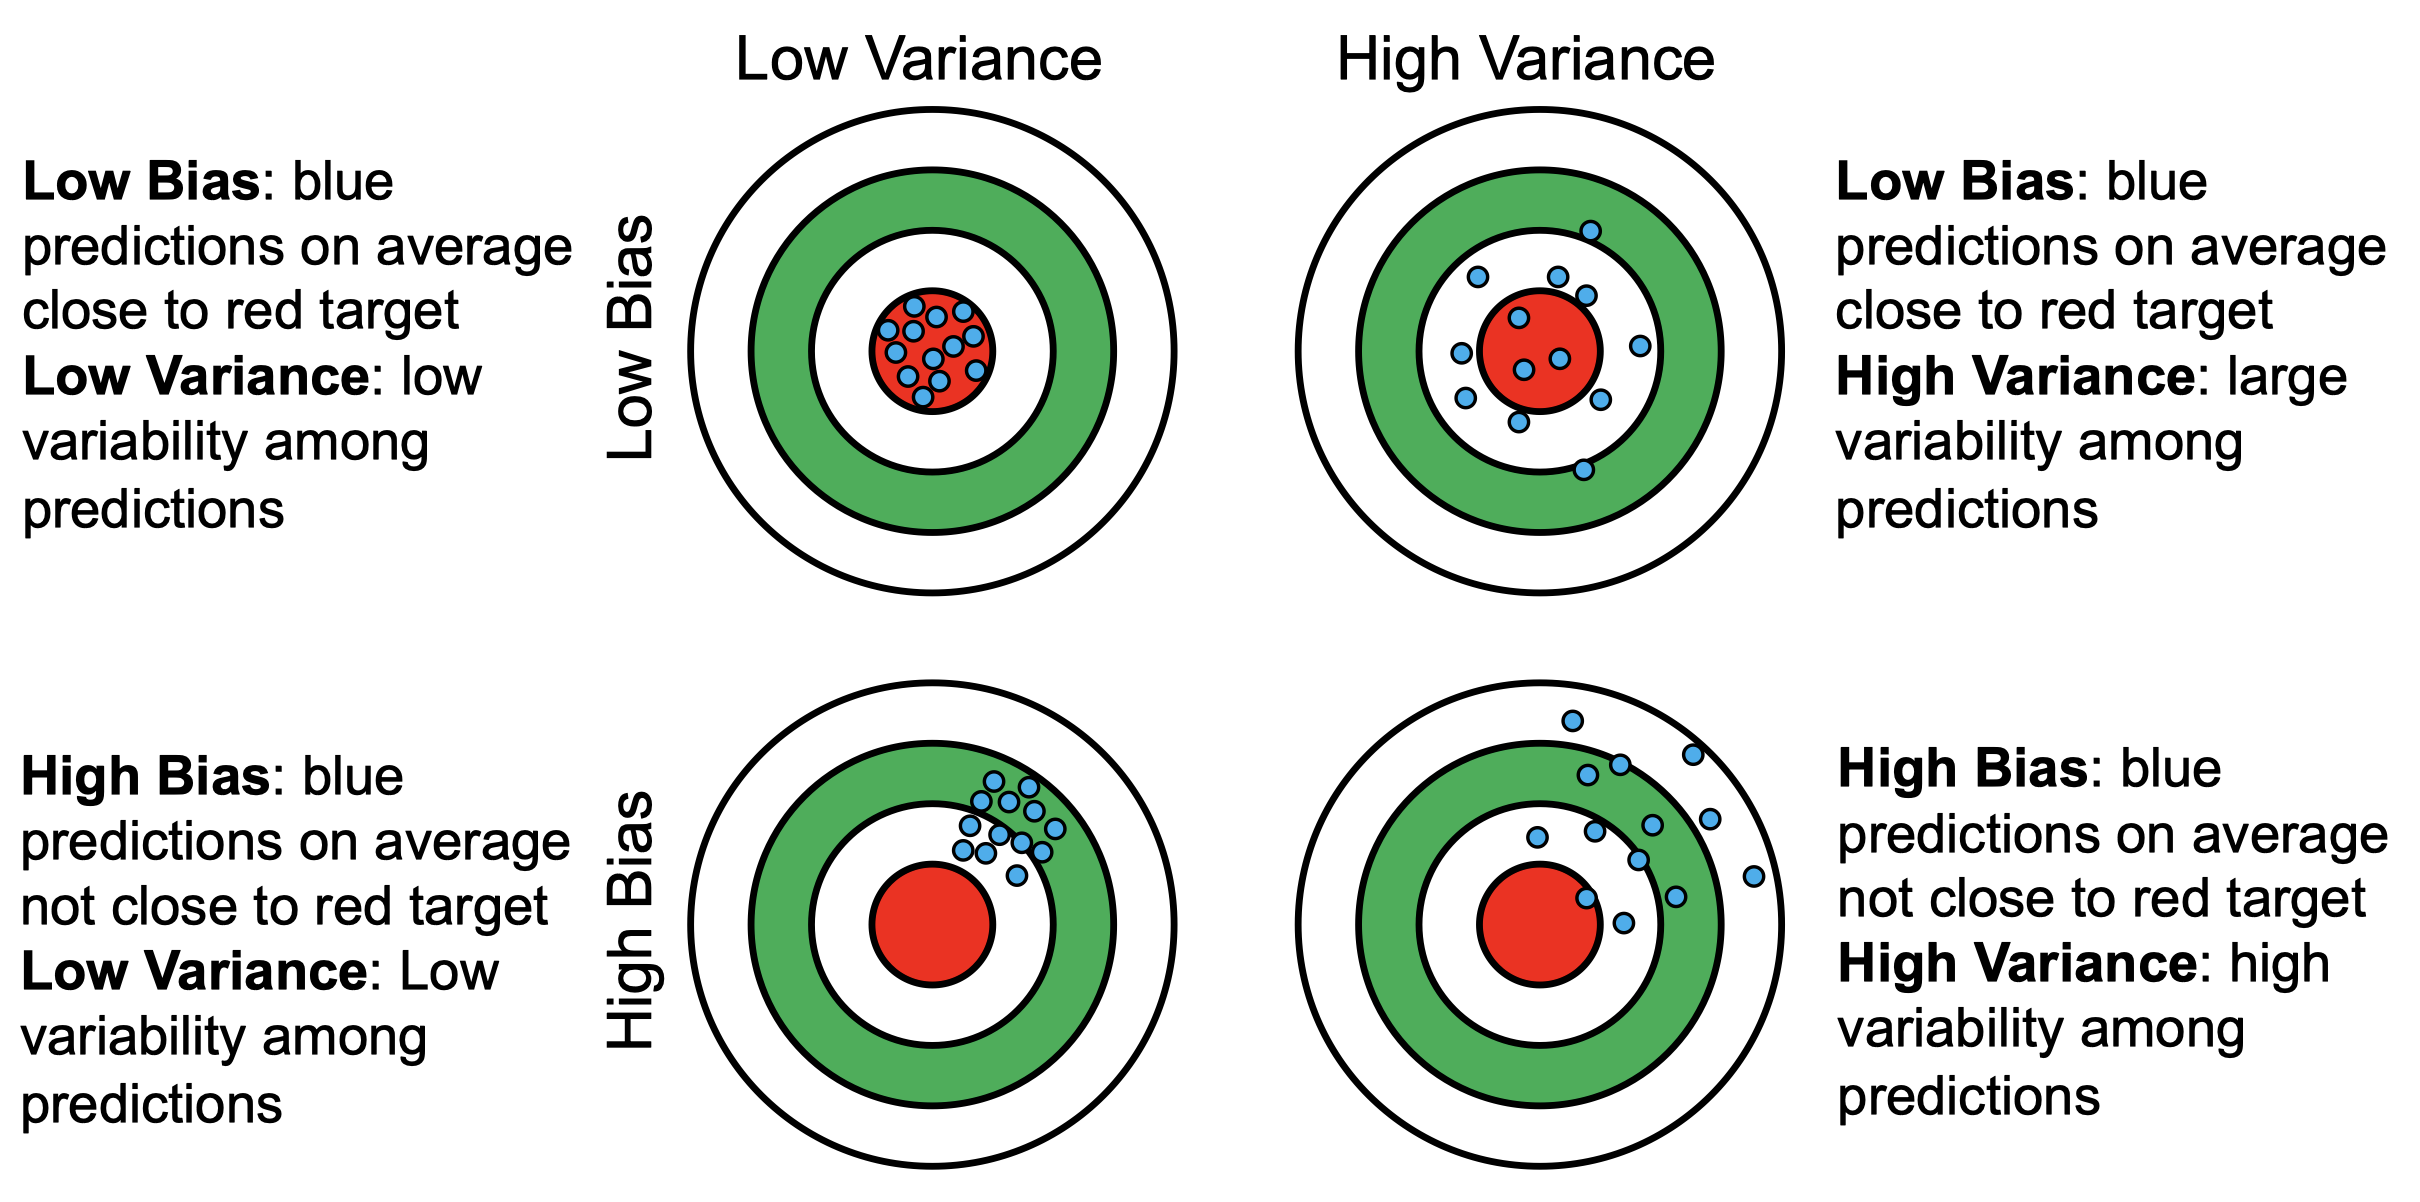
\includegraphics[width=1\linewidth]{image/bias_virance.png}
\end{figure}\\
\textbf{Test error} = Bias Squared + Variance + Irreducible Noise \\
\textbf{Variance} refers to variability of prediction models across different training sets \\
\textbf{Bias} refers to how well an average prediction model will perform\\
\textbf{Irreducible Noise} reflects the fact that even if we are perfect modelers, it might not be possible to predict target $y$ with 100\% accuracy from feature(s).
